\documentclass[10pt,journal]{IEEEtran}

\usepackage{cite}
\usepackage{amsmath}
\usepackage{amssymb}
\usepackage{booktabs}
\usepackage{array}
\usepackage{multirow}
\usepackage{siunitx}
\usepackage{pgfplots}
\usepackage{tikz}
\usepackage{xcolor}
\usepackage{balance}

\pgfplotsset{compat=1.18}
\sisetup{detect-all}

\newcommand{\rams}{RAMS}
\newcommand{\swas}{SWAS}

\begin{document}

\title{RAMS: Safety-Aware Model Switching for Edge Perception Across Heterogeneous Deployment Settings}

\author{Kushal~Khemani and Ajinkyaa~Lokhande}

\maketitle

\begin{abstract}
Edge perception systems often face a poor operating choice under load: keep a larger detector and violate latency targets, or drop to a smaller detector and lose vulnerable road user (VRU) sensitivity. This letter presents \rams{}, a runtime controller that monitors device pressure and switches among three warm YOLOv8 tiers using threshold, predictive, and safety-aware policies. \rams{} is evaluated across five deployment settings: Raspberry Pi 5 ONNX, two Windows x86 ONNX hosts, and Jetson Orin with both ONNX and TensorRT backends. The headline result is on Jetson Orin TensorRT under heavy load: \rams{} reduces mean latency by \textbf{5.6$\times$} relative to a fixed-MEDIUM policy while retaining \textbf{74\%} of that policy's tier-accuracy proxy. Real KITTI evaluation explains both the motivation and the boundary of this gain: Jetson VRU recall rises from \textbf{24.2\%} at NANO to \textbf{59.0\%} at MEDIUM, so the safety improvement is opportunistic rather than oracle-safe. The contribution is therefore a compact, deployable model-switching layer, an explicit safety-weighted policy metric, and a multi-setting deployment study that spans low-power CPU inference to embedded TensorRT acceleration.
\end{abstract}

\begin{IEEEkeywords}
edge AI, adaptive inference, model switching, safety-aware scheduling, TensorRT, Jetson, embedded perception
\end{IEEEkeywords}

\section{Introduction}
Edge perception is often deployed with one detector configuration chosen offline. That choice is brittle. A model sized for nominal conditions may violate latency budgets under CPU, memory, or thermal pressure, while a model sized for worst-case latency may under-detect the very events that justify a safety-aware pipeline. This tension is especially visible in embedded perception, where device heterogeneity is large and resource headroom can disappear quickly during sustained load.

Prior work addresses dynamic deep neural network execution through approximation, multi-tenant runtime adaptation, or device--edge partitioning~\cite{han2016mcdnn,fang2018nestdnn,kang2017neurosurgeon,li2018edgent}. Those systems are important precedents, but they do not directly target local safety-conditioned switching among warm detector tiers on heterogeneous edge hardware. The problem addressed in this letter is narrower and more deployment driven: given a single perception task already committed to local execution, can a runtime controller recover useful latency headroom while remaining conservative when VRU evidence is present?

\rams{} answers that question with a lightweight architecture. The runtime continuously monitors resource pressure, calibrates device-specific thresholds, and switches among NANO, SMALL, and MEDIUM YOLOv8 tiers without incurring model reload delays. In addition to threshold and predictive policies, \rams{} includes safety-aware policies that try to retain higher tiers when recent detections indicate that a pedestrian or cyclist may be present. To compare such policies with a single scalar, \rams{} defines a Safety-Weighted Accuracy Score (\swas{}) that rewards stronger tier choices when VRU detections occur.

This letter is written in the style that works for a compact embedded-systems submission: one sharp result supported by a small number of focused figures and tables. The headline result is on Jetson Orin TensorRT under heavy load: \rams{} reaches a \SI{3.41}{ms} operating point that is \textbf{5.6$\times$} faster than fixed-MEDIUM while retaining \textbf{74\%} of its tier-accuracy proxy. The rest of the paper explains how that result is obtained, why it is meaningful, and where its safety interpretation stops.

The paper makes three contributions.
\begin{enumerate}
\item It presents a deployable local controller for warm-tier model switching under edge resource pressure.
\item It introduces \swas{}, a compact metric for comparing safety-aware switching policies.
\item It evaluates the runtime across five deployment settings spanning Raspberry Pi 5 ONNX, two Windows x86 ONNX hosts, and Jetson Orin with both ONNX and TensorRT backends.
\end{enumerate}

\section{System Design}
\subsection{Runtime Structure}
The \rams{} runtime combines a resource monitor, a switching policy, and a warm model library. The resource monitor samples CPU utilization, memory pressure, and temperature-related indicators and compresses them into a normalized pressure score $R(t)\in[0,1]$. The switching policy maps that score, together with recent perception context, to one of three resident detector tiers. The model library holds YOLOv8n, YOLOv8s, and YOLOv8m in memory so that switching does not require model reload or graph reconstruction.

\begin{figure}[t]
\centering
\begin{tikzpicture}[node distance=2.2mm and 2.2mm, font=\scriptsize]
\tikzstyle{blk}=[draw, rounded corners=1pt, align=center, minimum height=8mm, minimum width=15mm]
\node[blk, fill=blue!7] (mon) {Resource\\monitor};
\node[blk, fill=green!8, right=of mon] (cal) {Calibration\\$R(t),\theta_{lo},\theta_{hi}$};
\node[blk, fill=orange!10, right=of cal] (pol) {Policy\\threshold / predictive\\safety / safety2};
\node[blk, fill=red!8, right=of pol, minimum width=23mm] (tiers) {Warm model tiers\\NANO / SMALL / MEDIUM};
\node[blk, fill=gray!10, below=of tiers, minimum width=23mm] (det) {Detections\\tier, latency, VRU flag};

\draw[->, thick] (mon) -- (cal);
\draw[->, thick] (cal) -- (pol);
\draw[->, thick] (pol) -- (tiers);
\draw[->, thick] (tiers) -- (det);
\draw[->, thick] (det.west) -| ++(-1.8,0) |- (pol.south);
\node[align=center, font=\scriptsize] at ($(pol)!0.5!(det)+(0,-1.0)$) {recent VRU evidence biases\\downgrade behavior};
\end{tikzpicture}
\caption{Compact \rams{} runtime. All tiers are warm in memory. Safety-aware policies feed recent VRU evidence back into tier selection instead of using pressure alone.}
\label{fig:arch}
\end{figure}

\subsection{Calibration and Policy Semantics}
Thresholds are calibrated per deployment setting rather than reused across devices. Let $\theta_{lo}$ and $\theta_{hi}$ be the low and high pressure thresholds after calibration. The threshold policy follows the piecewise rule
\begin{equation}
\tau(R)=
\begin{cases}
\text{MEDIUM}, & R < \theta_{lo}\\
\text{SMALL}, & \theta_{lo} \le R < \theta_{hi}\\
\text{NANO}, & R \ge \theta_{hi}.
\end{cases}
\end{equation}
Hysteresis suppresses rapid oscillation near decision boundaries. The predictive policy applies short-horizon smoothing so that imminent load spikes can trigger an earlier downgrade. The safety-aware policies inject a second signal: if recent detections suggest a VRU is present, the controller becomes more conservative about downgrading to weaker tiers. In practice, \texttt{safety} tends to preserve SMALL, while \texttt{safety2} is willing to hold MEDIUM longer.

This architecture is deliberately modest. It does not change network topology, retrain models online, or partition layers between devices. The point is to expose a low-overhead local decision layer that can be inserted above existing detector tiers and below application logic.

\subsection{Safety-Weighted Accuracy Score}
To compare policies using one number, \rams{} defines
\begin{equation}
\mathrm{SWAS}=\frac{1}{N(1+\beta)}\sum_{i=1}^{N} a_i \left(1+\beta v_i\right),
\end{equation}
where $a_i$ is the per-inference tier accuracy proxy, $v_i\in\{0,1\}$ denotes whether a VRU was detected, and $\beta=2$ in all reported runs. When $\beta=0$, \swas{} collapses to mean accuracy. When $\beta>0$, policies that retain stronger tiers during VRU-positive intervals receive a higher score than policies that uniformly chase latency.

This definition is useful precisely because \rams{} is not an accuracy-improvement paper. The metric is intended to compare switching behavior under a fixed tier library, not to replace live dataset evaluation. The live safety envelope is therefore reported separately through KITTI VRU recall in Exp.~8.

\section{Experimental Protocol}
\subsection{Deployment Settings}
Table~\ref{tab:devices} summarizes the five deployment settings used in this letter. A useful feature of the results is that calibration clearly differs across platforms. The laptop i7-1165G7 and Raspberry Pi 5 both converged to $(\theta_{lo},\theta_{hi})=(0.513,0.763)$, while Jetson Orin used lower thresholds $(0.362,0.612)$ and the i7-13700F desktop converged to $(0.300,0.542)$. This matters because \rams{} is not driven by a one-size-fits-all threshold choice.

\begin{table}[t]
\centering
\footnotesize
\setlength{\tabcolsep}{3.5pt}
\caption{Deployment settings and calibrated thresholds. The last two columns report the fastest heavy-load operating point observed for each setting and the dominant tier mix at that point.}
\label{tab:devices}
\begin{tabular}{>{\raggedright\arraybackslash}p{0.18\columnwidth} >{\raggedright\arraybackslash}p{0.12\columnwidth} c c c >{\raggedright\arraybackslash}p{0.23\columnwidth}}
\toprule
Setting & Backend & $\theta_{lo}$ & $\theta_{hi}$ & Heavy latency & Dominant tier mix \\
\midrule
Pi 5 & ONNX & 0.513 & 0.763 & 47.17 ms & 85\% N, 15\% S \\
i7-1165G7 & ONNX & 0.513 & 0.763 & 75.48 ms & 16\% N, 82\% S, 2\% M \\
i7-13700F & ONNX & 0.300 & 0.542 & 35.64 ms & 100\% S \\
Jetson Orin & ONNX & 0.362 & 0.612 & 127.52 ms & 100\% S \\
Jetson Orin & TRT & 0.362 & 0.612 & 3.41 ms & 99\% N, 1\% S \\
\bottomrule
\end{tabular}
\end{table}

\subsection{Reported Experiments}
The full repository contains a broader suite, but this paper uses only the experiments needed for a defensible compact letter. Exp.~5 provides heavy-load operating points for adaptive policies and fixed-tier baselines. Exp.~7 evaluates safety-aware switching with \swas{}. Exp.~8 performs live KITTI replay for VRU recall. Exp.~9 provides end-to-end real-inference latency across ONNX deployment settings. Table~\ref{tab:method} makes the reporting boundary explicit.

\begin{table}[t]
\centering
\footnotesize
\setlength{\tabcolsep}{3.2pt}
\caption{Methodological scope of the reported experiments. Rows that use tier-accuracy proxies are interpreted as within-setting policy comparisons, while Exp.~8 reports live detector behavior.}
\label{tab:method}
\begin{tabular}{>{\raggedright\arraybackslash}p{0.10\columnwidth} >{\raggedright\arraybackslash}p{0.18\columnwidth} >{\raggedright\arraybackslash}p{0.24\columnwidth} >{\raggedright\arraybackslash}p{0.36\columnwidth}}
\toprule
Exp. & Inputs & Accuracy source & Paper use \\
\midrule
5 & backend stress profile & tier-level mAP proxy & headline Jetson tradeoff \\
7 & KITTI image replay & proxy weighted by detected VRU events & safety-aware policy comparison \\
8 & KITTI images and labels & live VRU recall / miss rate & safety envelope \\
9 & KITTI image replay & no accuracy claim; latency and tier mix only & cross-setting deployment behavior \\
\bottomrule
\end{tabular}
\end{table}

KITTI~\cite{geiger2012kitti} is the primary dataset used in the paper. All tiers are implemented with Ultralytics YOLOv8~\cite{jocher2023yolov8}. The Jetson TensorRT path uses direct TensorRT inference and the corrected deployment backend from the final Jetson artifact set. Because evaluation budgets differ by device, the KITTI replay size is not identical across all runs; the important point for this letter is that live VRU recall trends are monotonic and consistent across hardware.

\section{Results}
\subsection{Headline Tradeoff on Jetson TensorRT}
Figure~\ref{fig:pareto} shows the heavy-load Jetson Orin TensorRT operating points from Exp.~5. The gray frontier is given by fixed-NANO, fixed-SMALL, and fixed-MEDIUM. The adaptive policies sit near that frontier, with \texttt{safety2} giving the most compelling point for this paper: \SI{3.41}{ms} mean latency at a weighted accuracy proxy of 0.373, compared to \SI{18.90}{ms} and 0.503 for fixed-MEDIUM. The resulting speedup is \textbf{5.6$\times$}.

\begin{figure}[t]
\centering
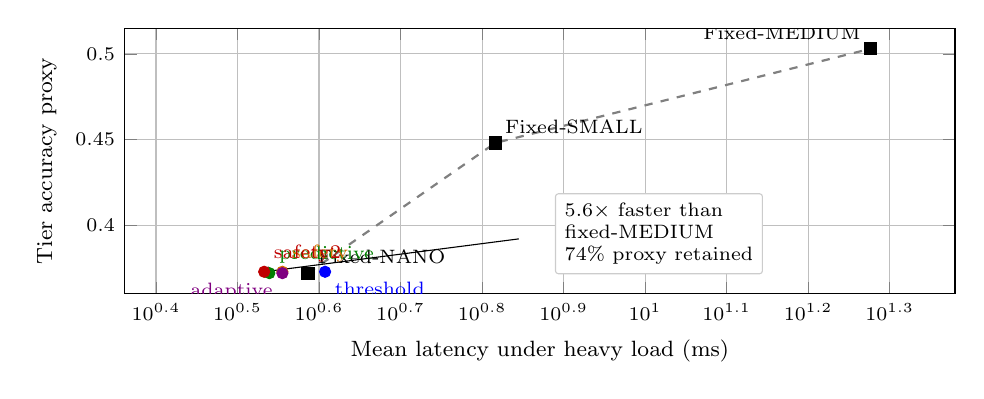
\begin{tikzpicture}
\begin{axis}[
width=\columnwidth,
height=1.95in,
xmode=log,
xmin=2.3, xmax=24,
ymin=0.36, ymax=0.515,
xlabel={Mean latency under heavy load (ms)},
ylabel={Tier accuracy proxy},
grid=major,
tick label style={font=\scriptsize},
label style={font=\footnotesize},
]
\addplot[dashed, gray, line width=0.8pt] coordinates {(3.86,0.372) (6.55,0.448) (18.90,0.503)};
\addplot[only marks, mark=square*, mark size=2.2pt, color=black] coordinates {(3.86,0.372) (6.55,0.448) (18.90,0.503)};
\addplot[only marks, mark=*, mark size=2.0pt, color=blue] coordinates {(4.05,0.3728)};
\addplot[only marks, mark=*, mark size=2.0pt, color=green!50!black] coordinates {(3.46,0.3720)};
\addplot[only marks, mark=*, mark size=2.0pt, color=orange!85!black] coordinates {(3.59,0.3728)};
\addplot[only marks, mark=*, mark size=2.0pt, color=violet] coordinates {(3.59,0.3720)};
\addplot[only marks, mark=*, mark size=2.0pt, color=red!75!black] coordinates {(3.41,0.3728)};

\node[font=\scriptsize, anchor=south west] at (axis cs:3.86,0.372) {Fixed-NANO};
\node[font=\scriptsize, anchor=south west] at (axis cs:6.55,0.448) {Fixed-SMALL};
\node[font=\scriptsize, anchor=south east] at (axis cs:18.90,0.503) {Fixed-MEDIUM};
\node[font=\scriptsize, anchor=north west, text=blue] at (axis cs:4.05,0.3728) {threshold};
\node[font=\scriptsize, anchor=south west, text=green!50!black] at (axis cs:3.46,0.3720) {predictive};
\node[font=\scriptsize, anchor=south west, text=orange!85!black] at (axis cs:3.59,0.3728) {safety};
\node[font=\scriptsize, anchor=north east, text=violet] at (axis cs:3.59,0.3720) {adaptive};
\node[font=\scriptsize, anchor=south west, text=red!75!black] at (axis cs:3.41,0.3728) {safety2};

\draw[->, thin] (axis cs:7.0,0.392) -- (axis cs:3.41,0.3728);
\node[font=\scriptsize, align=left, draw=gray!40, fill=white, rounded corners=1pt] at (axis cs:10.4,0.395) {5.6$\times$ faster than\\fixed-MEDIUM\\74\% proxy retained};
\end{axis}
\end{tikzpicture}
\caption{Jetson Orin TensorRT heavy-load operating points. The fixed-tier frontier is shown in gray. \texttt{safety2} is the best paper headline point because it preserves a measurable fraction of MEDIUM's tier quality while staying close to the low-latency frontier.}
\label{fig:pareto}
\end{figure}

This result is useful for two reasons. First, it shows that a local controller can recover most of the useful operating range between fixed-large and fixed-small inference without model reload cost. Second, it gives the paper a concrete embedded-systems number rather than a generic framework claim. The tradeoff is not free: \texttt{safety2} does not match fixed-MEDIUM accuracy. The result is instead that the controller can give back a large fraction of fixed-MEDIUM's utility at a latency point much closer to NANO.

\subsection{Safety-Aware Policy Behavior}
Exp.~7 provides the policy comparison that the latency-only Pareto view cannot show. Table~\ref{tab:exp7} summarizes Jetson TensorRT \swas{} values for moderate, heavy, and burst load. The key pattern is stable: the conservative policies only pay off when load is strong enough that tier choice matters. At moderate load, \texttt{safety2} achieves the highest \swas{} at 0.270, compared with 0.224 for threshold, predictive, safety, and adaptive. Under heavy and burst load, \texttt{safety2} continues to dominate, raising \swas{} from roughly 0.169 for latency-driven policies to approximately 0.249.

\begin{table}[t]
\centering
\footnotesize
\setlength{\tabcolsep}{3.0pt}
\caption{Jetson TensorRT Exp.~7 summary. Best \swas{} per load column is bold. The heavy and burst rows show the real behavior that motivates \rams{}: safety-aware policies spend more latency to preserve stronger tiers when VRU evidence is present.}
\label{tab:exp7}
\begin{tabular}{lrr|rr|rr}
\toprule
\multirow{2}{*}{Policy} & \multicolumn{2}{c|}{Moderate} & \multicolumn{2}{c|}{Heavy} & \multicolumn{2}{c}{Burst} \\
& \swas{} & ms & \swas{} & ms & \swas{} & ms \\
\midrule
threshold & 0.224 & 6.34 & 0.169 & 4.56 & 0.169 & 4.57 \\
predictive & 0.224 & 6.57 & 0.169 & 4.45 & 0.169 & 4.53 \\
safety & 0.224 & 6.60 & 0.223 & 7.28 & 0.223 & 7.42 \\
adaptive & 0.224 & 6.43 & 0.169 & 4.37 & 0.169 & 4.72 \\
safety2 & \textbf{0.270} & 13.62 & \textbf{0.249} & 13.05 & \textbf{0.249} & 13.18 \\
\bottomrule
\end{tabular}
\end{table}

Two observations matter. First, \swas{} is doing the intended work: it favors policies that retain stronger tiers when the scene is likely to be safety critical, not simply the policies with the smallest latency. Second, the gain is not created by an unrealistically large model being held all the time. The supporting traces show that \texttt{safety2} still degrades under pressure, but it does so more cautiously than the threshold and predictive rules.

\subsection{Safety Envelope: Real KITTI Recall}
The controller's safety story is bounded by detector recall. Figure~\ref{fig:recall} shows live KITTI VRU recall for the Jetson TensorRT and i7-1165G7 baselines. The trend is monotonic and consistent across hardware: larger tiers catch more VRUs, but even MEDIUM misses many events. On Jetson, recall rises from \textbf{24.2\%} at NANO to \textbf{59.0\%} at MEDIUM. On the laptop baseline, it rises from \textbf{24.4\%} to \textbf{58.7\%}.

\begin{figure}[t]
\centering
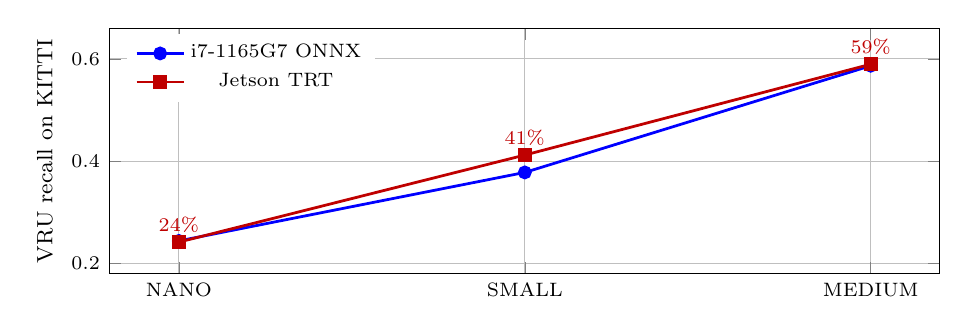
\begin{tikzpicture}
\begin{axis}[
width=\columnwidth,
height=1.85in,
xmin=-0.2, xmax=2.2,
ymin=0.18, ymax=0.66,
xtick={0,1,2},
xticklabels={NANO,SMALL,MEDIUM},
ylabel={VRU recall on KITTI},
grid=major,
tick label style={font=\scriptsize},
label style={font=\footnotesize},
legend style={font=\scriptsize, draw=none, at={(0.02,0.98)}, anchor=north west}
]
\addplot[blue, mark=*, line width=1.0pt] coordinates {(0,0.2441) (1,0.3780) (2,0.5866)};
\addlegendentry{i7-1165G7 ONNX}
\addplot[red!75!black, mark=square*, line width=1.0pt] coordinates {(0,0.2418) (1,0.4120) (2,0.5896)};
\addlegendentry{Jetson TRT}

\node[font=\scriptsize, text=red!75!black, anchor=south] at (axis cs:0,0.2418) {24\%};
\node[font=\scriptsize, text=red!75!black, anchor=south] at (axis cs:1,0.4120) {41\%};
\node[font=\scriptsize, text=red!75!black, anchor=south] at (axis cs:2,0.5896) {59\%};
\end{axis}
\end{tikzpicture}
\caption{Live KITTI VRU recall from Exp.~8. This is the paper's key safety limitation: \rams{} can only react to VRUs that the active detector tier actually sees.}
\label{fig:recall}
\end{figure}

This figure is central because it changes the interpretation of the whole system. \rams{} is \emph{opportunistic rather than oracle-safe}. If a VRU is missed by the current tier, no safety lock can fire. That limitation should not be hidden. At the same time, the figure justifies the runtime problem: moving from NANO to SMALL or MEDIUM does materially change the chance of seeing a VRU, so policy-level tier retention is not meaningless bookkeeping.

\subsection{Cross-Setting Deployment Behavior}
The multi-setting evaluation is one of the more distinctive parts of the project. Many adaptive-inference papers report one device. \rams{} is carried from low-power CPU-only inference to an embedded TensorRT target. Using the lowest-latency heavy-load operating point observed in each setting, the means are \SI{47.17}{ms} on Raspberry Pi 5 ONNX, \SI{75.48}{ms} on i7-1165G7 ONNX, \SI{35.64}{ms} on i7-13700F ONNX, \SI{127.52}{ms} on Jetson ONNX, and \SI{3.41}{ms} on Jetson TensorRT.

These numbers should not be overinterpreted as a uniform backend bakeoff, because Jetson TensorRT comes from the corrected Jetson heavy-load Pareto run while the ONNX settings come from Exp.~9. Still, the deployment story is useful. The same policy layer can be reused on a Raspberry Pi, an everyday laptop, a faster desktop host, and two Jetson backend modes. Even when the absolute latencies diverge substantially, the controller interface and policy semantics remain stable.

\section{Related Work}
Approximation and adaptive DNN execution on resource-constrained devices are well studied. MCDNN~\cite{han2016mcdnn} formulates approximate model scheduling for deep stream processing under resource constraints. NestDNN~\cite{fang2018nestdnn} introduces multi-capacity models and runtime resource-aware scheduling for continuous mobile vision. Neurosurgeon~\cite{kang2017neurosurgeon} and Edgent~\cite{li2018edgent} focus instead on partitioning inference across device and edge resources. \rams{} differs in target and granularity: it performs local warm-tier switching among full detector variants, includes an explicit safety-conditioned policy family, and emphasizes deployment across heterogeneous edge settings rather than cloud partitioning.

\section{Limitations and Conclusion}
\rams{} has three important limitations. First, its safety benefit is bounded by detector recall; it cannot protect against VRUs that the active tier never detects. Second, Exp.~5 and Exp.~7 use tier-level accuracy proxies, so those numbers should be interpreted as comparative policy scores within a setting rather than absolute cross-device accuracy measurements. Third, the five deployment settings are unified at the controller level but not at the exact harness level: the TensorRT headline point comes from the corrected Jetson TensorRT path, whereas the cross-setting ONNX numbers come from the Exp.~9 replay harness.

Those limits are real, but they do not erase the contribution. \rams{} offers a compact and reproducible model-switching layer for edge perception, shows that safety-aware policies can produce materially different operating points than latency-only rules, and reports a concrete Jetson TensorRT result that is easy to understand: \textbf{5.6$\times$} lower heavy-load latency than fixed-MEDIUM while retaining \textbf{74\%} of its tier-quality proxy. For an embedded-systems letter, that is the right level of claim: not a universal safety guarantee, but a deployable controller that quantifies when adaptive switching helps and what it buys.

\balance
\bibliographystyle{IEEEtran}
\bibliography{references}

\end{document}
